\vspace{2mm}
\section{Experiment}
Based on DLO-Lab tasks, we quantitatively evaluate three types of algorithms: (a) model-free reinforcement learning (MFRL) algorithms; (b) first-order model-based reinforcement learning (FO-MBRL) algorithms; and (c) trajectory optimization methods. We also conduct real-world experiments to verify the effectiveness of sim-to-real transfer.

\subsection{Benchmarked Methods}
\label{section:method_evaluation}
We conduct a comprehensive performance evaluation of various methods.
For MFRL algorithms, we evaluate 
Soft Actor-Critic (SAC)~\citep{haarnoja2018soft} and Proximal Policy Optimization (PPO)~\citep{schulman2017proximal}. 
For FO-MBRL algorithms, we evaluate Short-Horizon Actor-Critic (SHAC)~\citep{xuaccelerated} and Soft Analytic Policy Optimization (SAPO)~\citep{xingstabilizing}.
For trajectory optimization methods, we consider the Covariance Matrix Adaptation Evolution Strategy (CMA-ES)~\citep{cmaes} and gradient descent (GD).

\begin{figure*}[t]
    \centering
    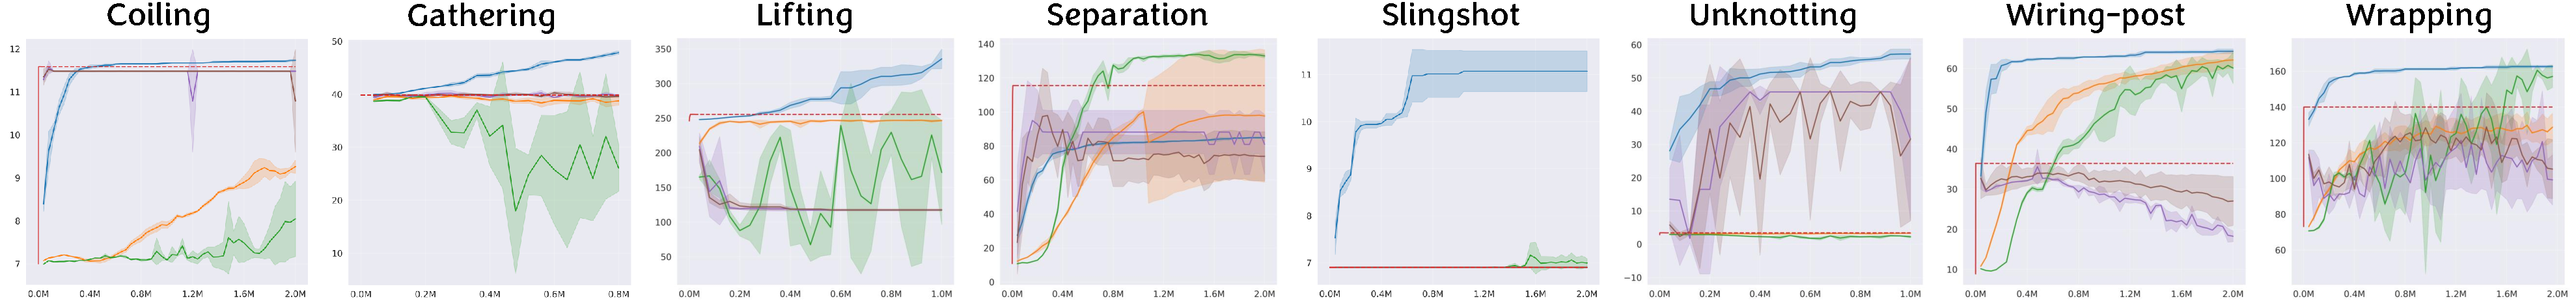
\includegraphics[width=\linewidth]{figs/curves_a_v2.pdf}
\vspace{-5mm}
    \caption{\textbf{DLO-Lab tasks training curves.} We report episodic return as a function of environment steps for the 8 fixed-horizon tasks. Color correspondence: \textcolor[HTML]{ff7f0e}{\bf PPO}, \textcolor[HTML]{2ca02c}{\bf SAC}, \textcolor[HTML]{9467bd}{\bf SHAC}, \textcolor[HTML]{8c564b}{\bf SAPO}, \textcolor[HTML]{d62728}{\bf GD}, and \textcolor[HTML]{1f77b4}{\bf CMA-ES}. For trajectory optimization methods, we plot the prefix maximum.}
    \label{fig:curve}
\end{figure*}

\begin{figure*}[t]
    \centering
    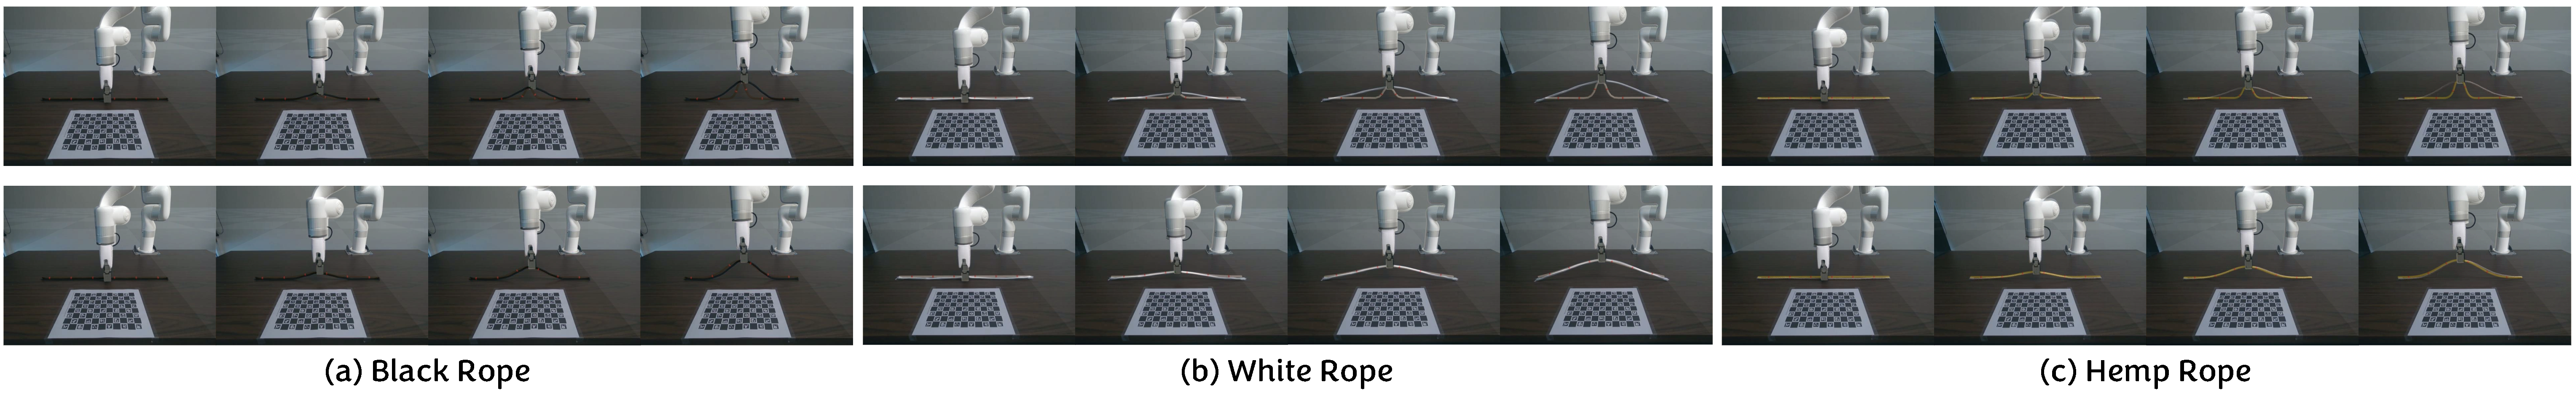
\includegraphics[width=1\linewidth]{figs/system_id_new.pdf}
\vspace{-5mm}
    \caption{\textbf{System identification results for three different ropes.}
    We overlay the real-world captures and simulation renderings in this figure. \emph{Top}: The simulation ropes with initial parameters. \emph{Bottom}: The simulation ropes with optimized parameters following system identification. Our identified parameters effectively capture the physical properties of the real-world DLOs.}
    \label{fig:system_id}
\vspace{-4mm}
\end{figure*}

\subsection{Results and Analysis}

\textbf{MFRL Algorithms}
As shown in~\Cref{tab:quantitative}, MFRL methods generally underperform compared to trajectory optimization given the same sampling budget. This performance gap is structural: trajectory optimization solves a simpler open-loop control problem, whereas MFRL attempts to learn a generalized closed-loop policy. The latter carries a significantly higher burden, requiring extensive exploration and a ``warm-up'' phase before the policy network converges to meaningful behaviors. As a result, in the sample-constrained regime of complex DLO manipulation, MFRL is less sample-efficient than direct trajectory optimization.

\textbf{FO-MBRL Algorithms}
Unlike standard MFRL, FO-MBRL methods, like SHAC and SAPO, leverage the simulator's differentiability to directly optimize policies using analytic gradients rather than relying solely on stochastic sampling. This provides a decisive advantage in contact-rich tasks where random exploration is insufficient. For instance, in the \textit{Unknotting} task, which requires precise topological manipulation, SHAC and SAPO achieve an episodic return of $\approx$ 46, whereas PPO and SAC fail to make progress (returns $\approx$ 3). However, FO-MBRL still lags behind sample-based trajectory optimization, \ie, CMA-ES, particularly in highly non-smooth or precisely coordinated tasks. This is because learning a closed-loop policy presents extra challenges; gradients can be noisy or misleading, particularly during intermittent contact and topological transitions.

\textbf{Trajectory Optimization}
The sample-based method, CMA-ES, achieves the strongest overall performance with reasonable sample efficiency, as shown in~\Cref{tab:quantitative} and~\Cref{fig:curve}. Its success can be attributed to two key factors. First, by bypassing the policy network, it avoids the optimization challenges associated with high-dimensional parameter spaces. Second, and more importantly, it does not depend on local gradient information, which can often be difficult or impossible to obtain for certain tasks (\eg, \textit{Lifting} and \textit{Slingshot}). In such tasks, the reward signal depends on the interaction between DLOs and rigid objects. If the DLO is not yet touching the object, the gradient of the reward with respect to the robot's action is effectively zero. CMA-ES is immune to these issues and can use massive parallelization in simulation to effectively explore the landscape, making it a robust choice for complex, multi-stage manipulation.

While gradient-based trajectory optimization, GD, is theoretically efficient, our results reveal two major issues in practice.
(1) Gradient inaccessibility: As noted above, in tasks requiring tool-use or indirect manipulation (\eg, \textit{Gathering}), useful gradients often do not exist until contact is established, making standard GD intractable without heuristic initialization.
(2) Non-smooth landscapes: Even when gradients are available, the optimization landscape for DLOs is notoriously rugged due to discontinuous contact events and self-collisions. As a result, GD frequently gets trapped in local optima, as evidenced by low scores on tasks such as \textit{Unknotting} (3.44) and \textit{Wiring-post} (36.40).
However, in tasks where the landscape is relatively smooth, and gradients are consistent—such as \textit{Coiling} and \textit{Separation}—GD demonstrates high efficacy. This validates the usefulness of differentiable simulation when the underlying physical dynamics are suitable for first-order optimization.

\subsection{Real-world Experiments}
\label{sec:real_world_exp}

\begin{figure*}[t]
    \centering
    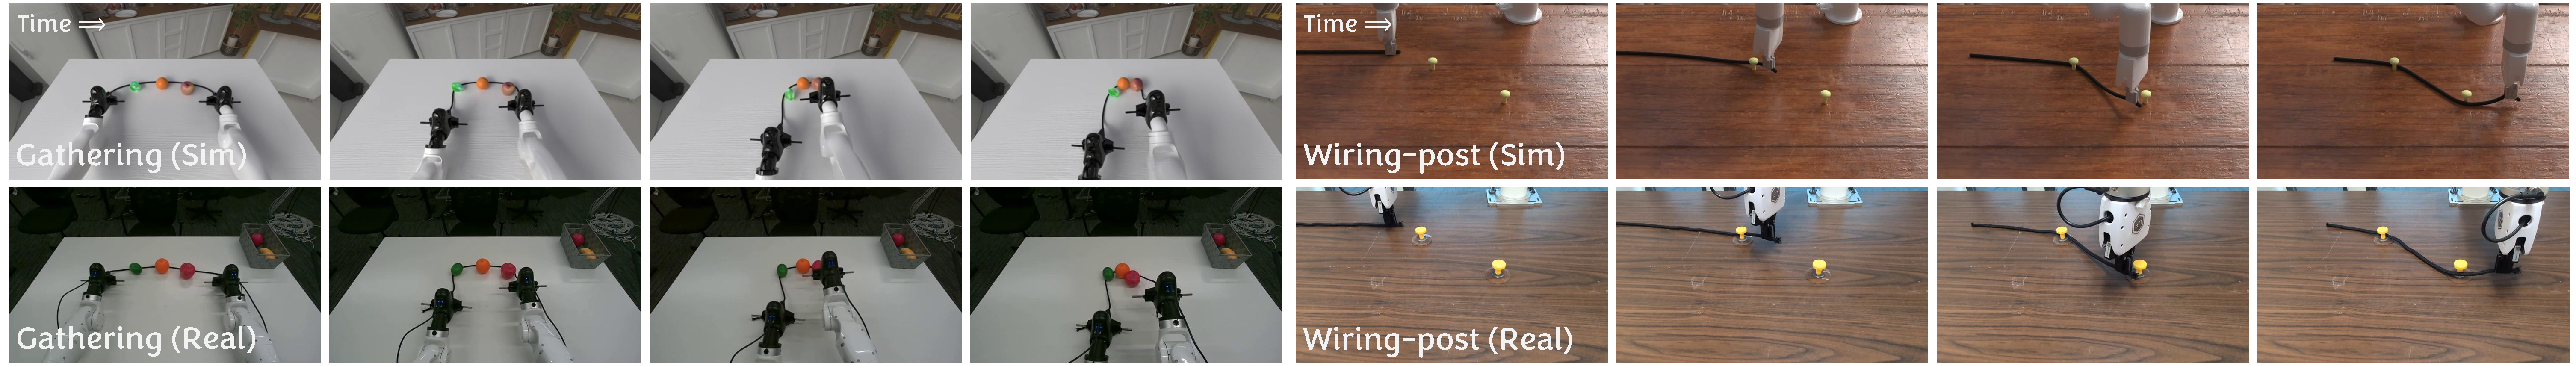
\includegraphics[width=\linewidth]{figs/real_demo_v2.pdf}
\vspace{-5mm}
    \caption{\textbf{Open-loop policy deployment results.}}
    \label{fig:open_loop}
\vspace{-2mm}
\end{figure*}


\begin{figure*}[t]
    \centering
    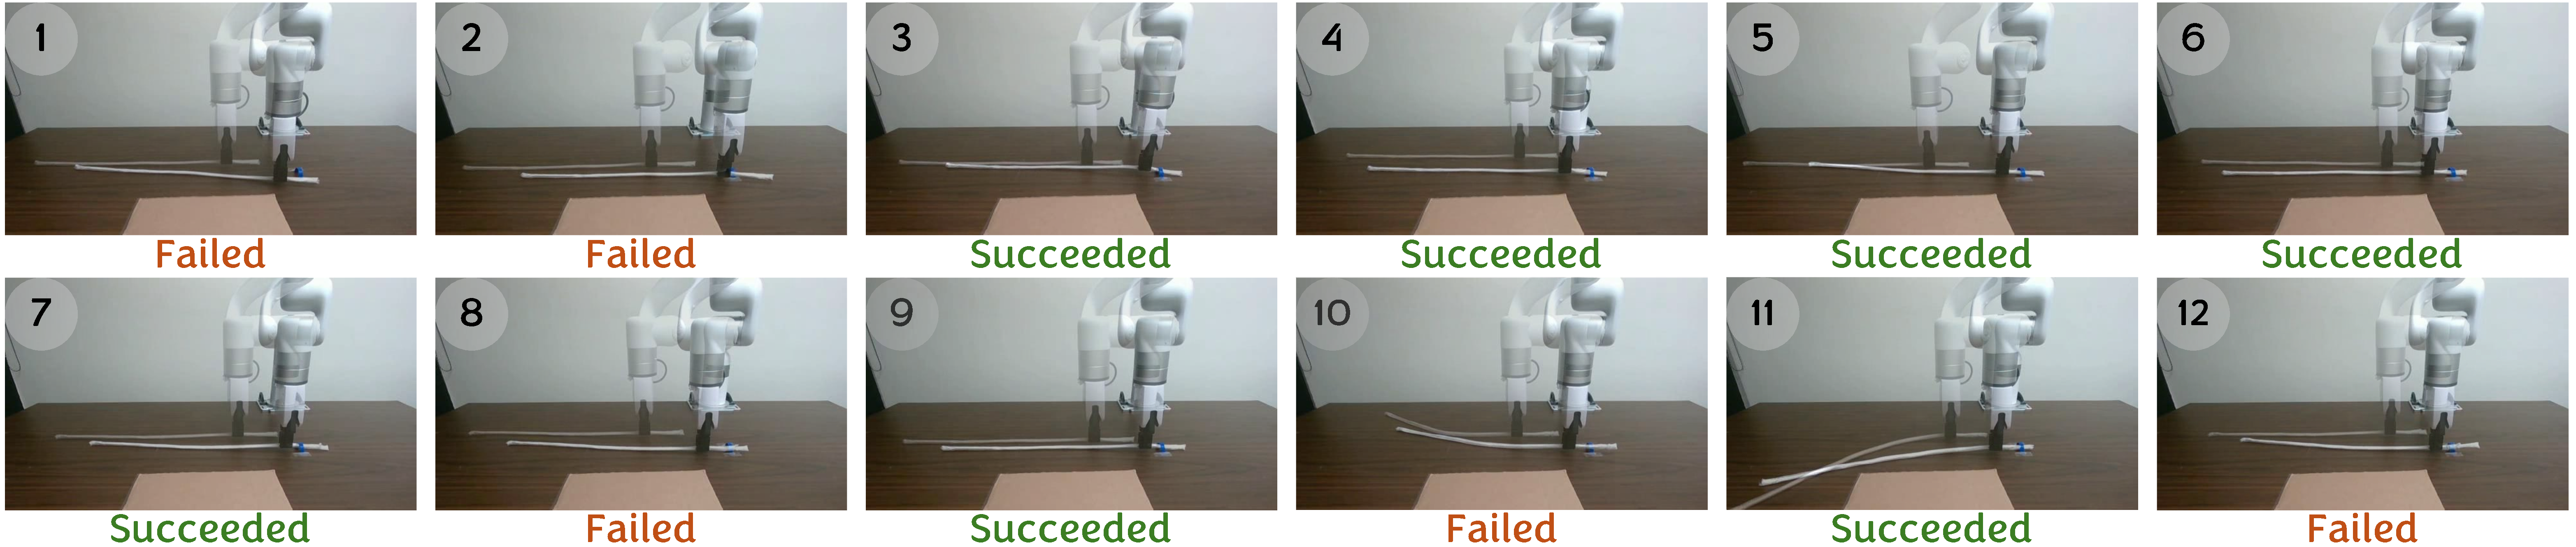
\includegraphics[width=\linewidth]{figs/real_world_v2.pdf}
\vspace{-4mm}
    \caption{\textbf{Closed-loop real-world policy deployment on the \textit{Wiring-ring} task.} We show the initial (semi-transparent) and final (solid) states for each of 12 trials. \textcolor[HTML]{3B7D23}{\bf Succeeded} and \textcolor[HTML]{C04F15}{\bf Failed} labels indicate the outcome of each trial.}
    \label{fig:close_loop}
\vspace{-4mm}
\end{figure*}


\textbf{System Identification}
\label{sec:details_system_id}
To bridge the gap between reality and simulation, we perform system identification to calibrate the physical parameters of the ropes used in our real-world experiments, including stretching and bending stiffness.
We use our extrinsically calibrated camera setup to overlay simulation renderings directly onto real-world video footage for visual verification. Thanks to our differentiable simulator, our goal is simply to minimize the projection error between simulation and reality: we project the simulated rope onto the image plane to obtain a binary segmentation mask, and compute its pixel-wise difference with the binary mask extracted from the real-world captures. Because the simulator is differentiable, the gradients of this pixel-level projection error are back-propagated through the physics timesteps directly to the underlying material parameters. \Cref{fig:system_id} illustrates the validation of this process. The top row shows the simulation behavior using uncalibrated initialization parameters, with a noticeable discrepancy between the simulated and real-world ropes, particularly during high-deformation lifting phases. In contrast, the bottom row shows the results after parameter optimization, in which the simulation closely tracks the real-world ropes' deformation, exhibiting accurate geometric alignment and dynamic response. This strong correspondence confirms that our identified parameters effectively capture the physical properties of the real-world DLOs.


\textbf{Open-loop Policy Deployment}
To validate the fidelity of our simulation, we conduct open-loop policy transfer on two tasks from DLO-Lab: (1) \textit{Gathering}, performed using a Marvin M6 bimanual manipulator, and (2) \textit{Wiring-post}, executed with an xArm. We employ a zero-shot strategy in which an open-loop policy is trained via sample-based trajectory optimization in simulation and deployed directly on the physical hardware without additional fine-tuning. The process begins with system identification to calibrate the black rope's material parameters within the simulation (\Cref{fig:system_id}(a)). During optimization, we incorporate the trajectory robustification technique proposed in SPIDER~\cite{pan2025spider} to enhance policy reliability against disturbances. As shown in~\Cref{fig:open_loop}, the trajectories generated in simulation are successfully executed on the physical setup, yielding outcomes comparable to the simulated results. These results confirm that our simulator captures sufficient physical realism to effectively bridge the sim-to-real gap.


\textbf{Closed-loop Policy Deployment}
To demonstrate that DLO-Lab supports closed-loop sim-to-real transfer, we train a closed-loop policy~\cite{schulman2017proximal} on the \textit{Wiring-ring} task and deploy it zero-shot on a physical xArm robot without additional fine-tuning. Here, \textit{Wiring-ring} requires threading a rope through a ring fixed to the table, demanding precise, reactive manipulation. To bridge the perception gap, the policy is trained with a simulated sensor model that mirrors the real-world HSV tracker. At each step, clean 3D points are sampled from the rope centerline and ring surface, projected to 2D image coordinates, dilated using 4-connected pixel neighbors to simulate the objects' physical width, and then unprojected back to 3D with Gaussian depth noise. 384 points are randomly drawn from this combined noisy cloud to form the observation, so rope and ring pixels are treated jointly without separation. At deployment, the same 384-point cloud is obtained by applying HSV color thresholding to the RGB camera feed and back-projecting the detected pixels using known camera extrinsics. The policy therefore receives two inputs at each step: (1) the 384-point 3D point cloud described above; and (2) the robot's proprioception. As shown in~\Cref{fig:close_loop}, the policy achieves 7 out of 12 successful completions ($\approx$58\%) with various initial rope positions. This result confirms that closed-loop policies trained in DLO-Lab can transfer to physical hardware and react responsively to the real-world rope state.

\label{section:experiment_real}
